% Created 2020-10-06 火 13:23
\documentclass{article}
\usepackage[utf8]{inputenc}
\usepackage[T1]{fontenc}
\usepackage{fixltx2e}
\usepackage{graphicx}
\usepackage{longtable}
\usepackage{float}
\usepackage{wrapfig}
\usepackage{rotating}
\usepackage[normalem]{ulem}
\usepackage{amsmath}
\usepackage{textcomp}
\usepackage{marvosym}
\usepackage{wasysym}
\usepackage{amssymb}
\usepackage{hyperref}
\tolerance=1000
\usepackage[margin=1.0in]{geometry}
\usepackage{mymacros}
\usepackage{amsmath,amssymb,amsthm}
\author{hisanobu-nakamura}
\date{\textit{<2020-02-26 月>}}
\title{Angular Momentum and Racah's formula}
\hypersetup{
  pdfkeywords={},
  pdfsubject={},
  pdfcreator={Emacs 25.3.2 (Org mode 8.2.10)}}
\begin{document}

\maketitle




\section{Introduction}
\label{sec-1}
This is a review of Racah's proof of the formula of the Clebsch-Gordan coefficients or Wigner's 3j-symbol and 6j-symbol.
\section{Angular Momentum Operators and $\mathfrak{su}(2)$ Representation}
\label{sec-2}
$J_x,J_y,J_z \in \mathfrak{su}(2)$
\begin{equation}
\label{}
[J_i,J_j] = i\epsilon_{ijk}J_k
\end{equation}
The Casimir operator $J ^2 = J_x^2 + J_y^2 + J_z^2$ and the ladder operators $J_{\pm}=J_x\pm iJ_y$
\begin{eqnarray}
\left[J^2,J_i\right] &=& 0\\
\left[J_z,J_{\pm}\right] & = & \pm J_{\pm} \\
\left[ J_+,J_- \right] &=& 2J_z\\
J^2 & = & J_-J_+ +J_z^2 + J_z \\
    &=& J_+J_- +J_z^2 - J_z 
\end{eqnarray}
Let $V$ be a finite dimensional vector space over $\C$ and $\varphi:\mathfrak{su}(2) \rightarrow \mathbf{End}(V)$ be its associated representation.
The Casimir operator $J ^2$ and $J_{z}$ commute, so there are simultaneous egenvectors of the operators. 
It can be shown that, by the finiteness of the dimension $V$, $J_{z}$ has a maximal eigenvalue $j$, which is called the \textbf{spin} of the representation.
So it is plausible to denote the representation space as $V_{j}$. And it can be shown that the simultaneous eigenvalue of $J ^2$ is $j(j+1)$ and invariant of the eigenvalue of $J_{z}$.
 Let us write an eigenvector of $J_{z}$ with the eigenvalue $m$ as $\ket{jm} \in V_{j}$. Then, in summary, we have
\begin{equation}
\label{}
J^2\ket{jm} = j(j+1)\ket{jm}, \quad J_z\ket{jm} = m\ket{jm}.
\end{equation}

\section{The ladder operators' coefficients}
\label{sec-3}
\begin{eqnarray}
J_{+}\ket{jm} & = & \sqrt{j(j+1) - m(m+1)}\ket{jm+1} \\
& = & \sqrt{(j- m)(j+ m +1)}\ket{jm+1}\\
J_{-}\ket{jm} & = & \sqrt{j(j+1) - m(m-1)}\ket{jm-1} \\
& = & \sqrt{(j+ m)(j- m +1)}\ket{jm-1}
\end{eqnarray}
It is useful to write $\ket{jm}$ in terms of $(J_{-})^k \ket{jj}$. So, let us rewrite the coefficients in simpler notation;
\begin{equation}
\label{ }
J_{-} \ket{jj-(k-1)} = f(j,k)\ket{j j-k}
\end{equation}
where
\begin{eqnarray*}
f(j,k) := \sqrt{k(2j - k +1)} \;,1\le k \le 2j
\end{eqnarray*}
\begin{figure}[htb]
\centering
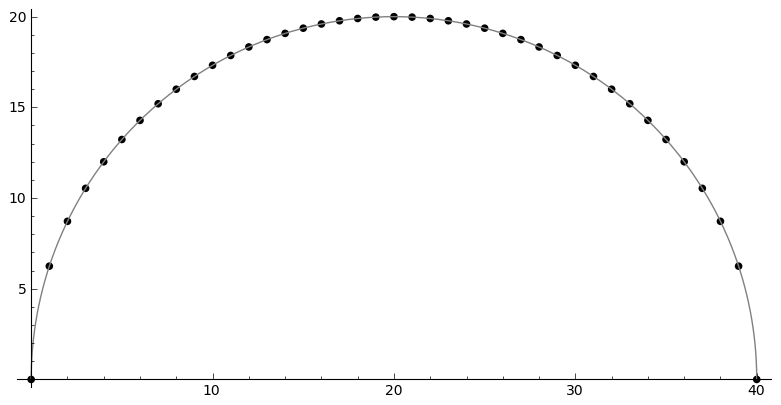
\includegraphics[width=80mm]{./images/ladder_coeff.png}
\caption{\label{fig:ladder_coeff}The graph of $f(j=\frac{39}{2},k)$ where $k$ is the horizontal axis.}
\end{figure} \\
We also have
\begin{equation}
\label{ }
J_{+}\ket{j j-k} = f(j,k)\ket{j j-k+1}
\end{equation}
Note that $D := 2j+1$ is the dimension of the $j$-th representation space.\\
Hence
\begin{eqnarray}
(J_{-})^k \ket{jj} & = & F(j,k) \ket{j j-k}
\end{eqnarray}
where $F(j,k) = \prod_{i=1}^{k} f(j,i)$ and evaluated as,
\begin{eqnarray}
F(j,k)  & = & \sqrt{k(2j+1 - k)(k-1)(2j+1 -(k-1))\times \cdots \times 2\cdotp (2j+1 -2) \cdot 1 \cdot (2j+1 -1)} \nonumber\\
        & = & \sqrt{k(D - k)(k-1)(D -(k-1))\times \cdots \times 2\cdotp (D -2) \cdot 1 \cdot (D -1)}\nonumber\\
        & = & \sqrt{\frac{k!(2j)!}{(2j -k)!}} = k!\sqrt{_{2j}C_{k}}
\end{eqnarray}
and $F(j,0)=1$
\section{Recursion Relations for Clebsch-Gordan coefficients}
\label{sec-4}
The tensor product of two representation space $V_{j_{1}} \otimes V_{{j_{2}}$ decomposes into the direct sum of irreducible representations $V_{J}$ where $|j_{1} - j_{2}| \le J \le j_{1} +j_{2}$ as
\begin{equation}
V_{j_{1}} \otimes V_{j_{2}} = V_{|j_{1} - j_{2}|} \oplus \cdots \oplus V_{j_{1} +j_{2}}
\end{equation}
\begin{figure}[htb]
\centering
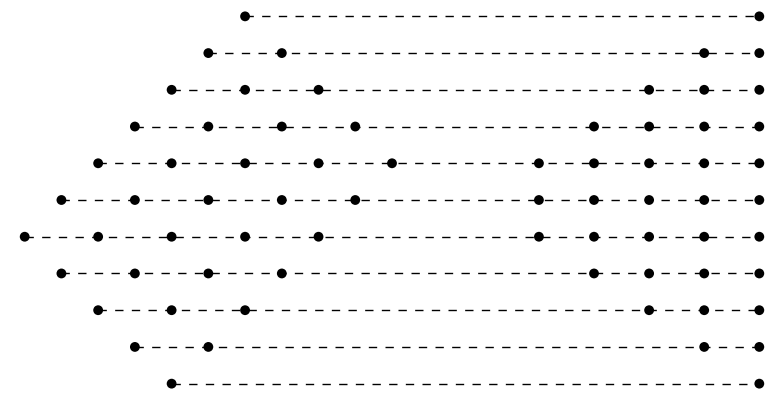
\includegraphics[width=80mm]{./images/j_grids.png}
\caption{\label{fig:j-grids}Correspondence between the tensor product $V_{j_{1}}\otimes V_{j_{2}}$ and $V_{J}$ ($j_{1}=3,j_{2}=2$).}
\end{figure}\\
One of the elements in $\ket{j_1j_{2}JM} \in V_{J}$ is expandable by the tensor basis of $\ket{j_1 j_2 m_1 m_2} := \ket{j_1 m_1} \otimes \ket{j_2 m_2} \in V_{j_{1}} \otimes V_{j_{2}}$ as
\begin{equation}
\label{}
\ket{j_1j_2 JM} = \sum_{m_1,m_2} \ket{j_1 j_2m_1m_2}\inn{j_1j_2m_1m_2}{JM}.
\end{equation}
The coefficients $\inn{j_1j_2m_1m_2}{JM}$ are called \textbf{Clebsch-Gordan coefficients} and they can be recursively calculated by the following formulae:
Apply $J_+ = j_{1+} + j_{2+}$ take inner product with $\bra{j_1j_2m_1m_2}$
\begin{eqnarray}
&&\sqrt{J(J+1) - M(M+1)}\inn{j_1 j_2 m_1 m_2}{JM+1}  \nonumber\\
&&=  \sqrt{j_1(j_1+1) - m_1(m_1-1)}\inn{j_1 j_2 m_1-1 m_2}{JM} +   \sqrt{j_2(j_2+1) - m_2(m_2-1)}\inn{j_1 j_2 m_1 m_2-1}{JM}\nonumber\\
\end{eqnarray}
and $J_- = j_{1-} + j_{2-}$ 
\begin{eqnarray}
&&\sqrt{J(J+1) - M(M-1)}\inn{j_1 j_2 m_1 m_2}{JM-1}  \nonumber\\
&&=  \sqrt{j_1(j_1+1) - m_1(m_1+1)}\inn{j_1 j_2 m_1+1 m_2}{JM} +   \sqrt{j_2(j_2+1) - m_2(m_2+1)}\inn{j_1 j_2 m_1 m_2+1}{JM}\nonumber\\
\end{eqnarray}

\section{Explicit formulae for Clebsch-Gordan coefficinets}
\label{sec-5}
\subsection{$\inn{j_1j_2m_1m_2}{JM}$}
\label{sec-5-1}
Define $d=j_1+j_2 -J$, ($j_1 \ge j_2$ and $0\le d \le 2j_2$), and $L = J-M$. Let us determine the coefficients of the top spin state
\begin{eqnarray}
\ket{JJ}  &=&  a_0\ket{j_1j_1}\ket{j_2j_2-d} + a_1\ket{j_1j_1-1}\ket{j_2j_2-d+1} + \cdots + a_d\ket{j_1j_1-d}\ket{j_2j_2} \nonumber\\
 & = & \sum_{i=0}^{d} a_i\ket{j_1j_1-i}\ket{j_2j_2-d+i}
\end{eqnarray}
by imposing the top spin condition
\begin{equation}
\label{ }
J_{+}\ket{JJ}  =  0 \implies a_{i+1}=-\frac{f(j_2,d-i)}{f(j_1,i+1)}a_i \quad (i=0,\ldots,d-1),
\end{equation}
which means
\begin{eqnarray}
 a_{i} & = & -\frac{f(j_2,d-(i-1))}{f(j_1,i)}a_{i-1} \quad (i=1,\ldots,d)\\
       & = & (-1)^i\frac{f(j_2,d-(i-1))f(j_2,d-(i-2)) \cdots f(j_2,d-1)f(j_2,d)}{f(j_1,i)f(j_1,i-1) \cdots f(j_1,2)f(j_1,1)}a_{0} \\
       & = & (-1)^i\frac{F(j_2,d)}{F(j_1,i)F(j_2,d-i)} a_{0} 
\end{eqnarray}
Here $F(j_2,0)=1$.
\subsection{Derivation of Racah's formula}
\label{sec-5-2}
Normalisation condition $\inn{JJ}{JJ}=1$ yields
\begin{eqnarray}
 \frac{1}{a_{0}^2} & = & \sum_{i=0}^{d}\frac{F(j_2,d)^2}{F(j_1,i)^2F(j_2,d-i)^2}\\
                   & = & 1+\left[ \frac{f(j_2,d)}{f(j_1,1)} \right]^2+ \cdots + \left[\frac{f(j_2,d-(i-1))f(j_2,d-(i-2)) \cdots f(j_2,d-1)f(j_2,d)}{f(j_1,i)f(j_1,i-1) \cdots f(j_1,2)f(j_1,1)}\right]^2 + \nonumber\\
                   & &   \cdots + \left[\frac{F(j_2,d)}{F(j_1,d)} \right]^2 \nonumber\\
                   & = & \frac{1}{F(j_1,d)^2} \bigg\{ (D_1-d)\cdot d\cdots (D_1-2)\cdot 2 \cdot (D_1 -1) \cdot 1 +(D_1-d)\cdot d\cdots (D_1-2)\cdot 2 \cdot (D_2-d)\cdot d + \nonumber\\
                   & &   \cdots + (D_1-d)\cdot d\cdots (D_1-i-1)\cdot (i+1) \cdot (D_2 -(d-i+1)) \cdot (d-i+1) \cdots (D_2-d)\cdot d + \cdots \bigg\} \nonumber\\
                   & = & \frac{1}{F(j_1,d)^2} \bigg\{ \frac{(d!)^2}{d!}(D_1-d)\cdot  (D_1-2)\cdot  (D_1 -1)  + \frac{(d!)^2}{1!(d-1)!}(D_1-d)\cdots (D_1-2) \cdot (D_2-d) + \nonumber\\
                   & &   \cdots + \frac{(d!)^2}{i!(d-i)!}(D_1-d)\cdot (D_1-i-1) \cdot (D_2 -(d-i+1)) \cdots (D_2-d) + \cdots \bigg\} \nonumber
\end{eqnarray}
Writing 
\begin{eqnarray}
 G_i(j_1,j_2,d) &:=& \frac{F(j_1,d)F(j_2,d)}{F(j_1,i)F(j_2,d-i)}, \\
                & = & \sqrt{\frac{(d!)^2}{(d-i)!i!}(D_2 - d)(D_2 -d-1)\cdots(D_2 - d -i+1)(D_1 - d) \cdots (D_1 - i +1)} \nonumber
\end{eqnarray}
Or, substituting  $d = j_1+j_2 -J$, this can be written as
\begin{eqnarray}
G_i(j_1,j_2,j_1+j_2 -J) & = & (-1)^i\sqrt{\frac{((j_1+j_2 -J)!)^2}{(j_1+j_2-J-i)!i!}\frac{(-j_1+j_2+J)!(j_1+J-j_2)!}{(-j_1+j_2+J -i)!(2j_1  - i)!}}. \nonumber
\end{eqnarray}
In terms of these $G_i$'s, the coefficients $a_i$ become
\begin{equation}
\label{ }
a_i = (-1)^i\frac{G_i(j_1,j_2,d)}{\sqrt{\sum_{i=1}^{d}G_i(j_1,j_2,d)^2}}.
\end{equation}
We want to know the normalising coefficient $N := \frac{1}{\sqrt{\sum_{i=1}^{d}G_i(j_1,j_2,d)^2}}$. In order to simplify the sum
\begin{eqnarray}
\sum_{i=1}^{d}G_i(j_1,j_2,d)^2 &=& \sum_{i=1}^{d}\frac{F(j_1,d)^2F(j_2,d)^2}{F(j_1,i)^2F(j_2,d-i)^2} \nonumber \\
 & = & \frac{(d!)^2}{(2j_1-d)!(2j_2-d)!} \sum_{i=1}^{d}\frac{(2j_1-i)!(2j_2-d+i)!}{i!(d-i)!},
\end{eqnarray} 
we use a formula due to Racah (mentioned in Messiah\cite{Messiah})
\begin{equation}
\label{eq:general_binomial_coeff}
\sum_{s} \frac{(a+s)!(b-s)!}{(c+s)!(d-s)!} = \frac{(a+b+1)!(a-c)!(b-d)!}{(c+d)!(a+b-c-d+1)!}.
\end{equation}
with $a\ge c, b\ge d \ge 0$, where the sum is taken over $-c\le s \le d$.\\
Now substituting $a = 2j_2-d, b = 2j_1, c=0, d= d$, we obtain
\begin{equation}
\label{ }
N = \sqrt{\frac{(2j_2-2d+2j_1+1)!}{d!(2j_2-d+2j_1+1)!}} = \sqrt{\frac{(2J+1)!}{(j_1+j_2 -J)!(j_1+j_2+J+1)!}}
\end{equation}
\begin{eqnarray}
a_i & = &  (-1)^iNG_i(j_1,j_2,d)\nonumber
\end{eqnarray}
Now, by multiplying the top-spin state with the ladder operators L times, we obtain the state $\ket{JM}$ with $M=J-L$
\begin{eqnarray}
J_{-}^L\ket{JJ} & = & (j_{1-} + j_{2-})^L\sum_{h=0}^{d}a_h\times \ket{j_1j_1 -h}\ket{j_2j_2-d+h} \nonumber\\
F(J,L)\ket{JJ-L}&=& \sum_{h=0}^{d}a_h\sum_{l=0}^{L}{}_LC_{l}\frac{F(j_1,h+l)F(j_2,(L+d)-(l+h))}{F(j_1,h)F(j_2,d-h)}\ket{j_1j_1 -(h + l)}\ket{j_2j_2 - (L+d) + (h + l)}  \nonumber\\
\ket{JJ-L}&=& \frac{1}{F(J,L)} \sum_{k=0}^{L+d} \left[ \sum_{k=h+l,\substack{0\le h \le d\\0\le l \le L}} a_h \times {}_LC_{l}\frac{F(j_1,k)F(j_2,K-k)}{F(j_1,h)F(j_2,d-h)}\right] \ket{j_1j_1 -k}\ket{j_2j_2 - K + k}  \nonumber\\
         &=& \frac{N}{F(J,L)} \sum_{k=0}^{L+d} F(j_1,k)F(j_2,K-k) \left[ \sum_{\substack{k=h+l\\0\le h \le d\\0\le l \le L}} \frac{ (-1)^h {}_LC_{l}G_h(j_1,j_2,d) }{F(j_1,h)F(j_2,d-h)}\right] \ket{j_1j_1 -k}\ket{j_2j_2 - K + k}  \nonumber
\end{eqnarray}
where $K=L+d = J- M + j_1 + j_2 -J = j_1 +j_2 -M$. Now, consider the coefficients of $\ket{j_1j_1 -k}\ket{j_2j_2 - K + k}$
\begin{eqnarray}
B_k & := & F(j_1,k)F(j_2,K-k) \left[ \sum_{\substack{k=h+l\\0\le h \le d\\0\le l \le L}} \frac{ (-1)^h {}_LC_{l}G_h(j_1,j_2,d) }{F(j_1,h)F(j_2,d-h)}\right] \nonumber\\
 & = & \sqrt{\frac{k!(K-k)!}{(2j_1 -k)!(2j_2-K+k)!}}  \sum_{\substack{k=h+l\\0\le h \le d\\0\le l \le L}}  (-1)^h {}_LC_{l}\sqrt{\frac{(2j_1-h)!(2j_2-d+h)!(d!)^2(2j_1-h)!(2j_2-d+h)!}{h!(d-h)!(2j_1-d)!(2j_2-d)!h!(d-h)!}}  \nonumber \\
 &=& \sqrt{\frac{k!(K-k)!}{(2j_1 -k)!(2j_2-K+k)!(2j_1-d)!(2j_2-d)!}} L!d!\sum_{\substack{k=h+l\\0\le h \le d\\0\le l \le L}}  (-1)^h \frac{(2j_1-h)!(2j_2-d+h)!}{h!(d-h)!l!(L-l)!} \nonumber 
\end{eqnarray}
The coefficient outside the sum, in terms of $j_1,j_2,J,m_1,m_2,M$, using the relations $K=L+d = J- M + j_1 + j_2 -J = j_1 +j_2 -M$, $k=j_1-m_1$, is
\begin{equation}
\label{ }
\sqrt{\frac{(j_1-m_1)!(j_2+m_1 -M)!}{(j_1 + m_1)!(j_2-m_1 +M )!(j_1-j_2 +J)!(j_2-j_1 +J)!}} (J-M)!(j_1+j_2-J)!
\end{equation}
Multiplying by $\frac{N}{F(J,J-M)}$
\begin{eqnarray}
&&\sqrt{\frac{(2J+1)(j_1+j_2 -J)!}{(j_1-j_2 +J)!(j_2-j_1 +J)!(j_1+j_2+J+1)!}\frac{(j_1-m_1)!(j_2-m_2)!(J+M)!(J-M)!}{(j_1 + m_1)!(j_2+m_2 )!}} \nonumber\\
&& = \sqrt{(2J+1)}\sqrt{\Delta(j_1j_2J)}\sqrt{(j_1 + m_1)!(j_1-m_1)!(j_2+m_2 )!(j_2-m_2)!(J+M)!(J-M)!} \nonumber\\
&&\times\frac{1}{(j_1-j_2 +J)!(j_2-j_1 +J)!(j_1 + m_1)!(j_2+m_2 )!}
\end{eqnarray}
where we have defined
\begin{equation}
\label{ }
\Delta(abc) := \frac{(a+b-c)!(b+c-a)!(c+a-b)!}{(a+b+c+1)!}.
\end{equation}
Now, we want to simplify the sum
\begin{eqnarray}
&&\sum_{\substack{k=h+l\\0\le h \le d\\0\le l \le L}}  (-1)^h \frac{(2j_1-h)!(2j_2-d+h)!}{h!(d-h)!l!(L-l)!}
\end{eqnarray}
furthermore. Putting $k = j_1- m_1$, $d= j_1 + j_2 -J$ back, we have
\begin{eqnarray}
&&\sum_{\substack{k=h+l\\0\le h \le d\\0\le l \le L}}  (-1)^h \frac{(2j_1-h)!(2j_2-d+h)!}{h!(d-h)!l!(L-l)!} \nonumber\\ 
&&=\sum_{\substack{l}} (-1)^{j_1 -m_1 -l} \frac{(j_1+m_1+l)!(j_2+J-m_1-l)!}{l!(j_1-m_1-l)!(j_2-J+m_1+l)!(J-M-l)!} \nonumber
\end{eqnarray}
and the sum in the last line is taken over all the values of $l$ with which all the factrial terms containing $l$ makes sense. In order to do so, we are going to use the following formula
\begin{equation}
\label{eq:factorial-triad}
\frac{a!}{b!c!}= \sum_{s} \frac{(a-b)!(a-c)!}{s!(a-b-s)!(a-c-s)!(b+c-a+s)!}.
\end{equation}
Now
\begin{eqnarray}
\label{eq:2-var-sum}
& &\sum_{\substack{l}} (-1)^{j_1 -m_1 -l} \frac{(j_1+m_1+l)!(j_2+J-m_1-l)!}{l!(j_1-m_1-l)!(j_2-J+m_1+l)!(J-M-l)!}   \nonumber\\
& = &  \sum_{\substack{l}} (-1)^{j_1 -m_1 -l} \frac{(j_1+m_1+l)!}{l!(j_2-J+m_1+l)!}\cdot\frac{(j_2+J-m_1-l)!}{(J-M-l)!(j_1-m_1-l)!} \nonumber\\
& = &  \sum_{\substack{l,l_1}} (-1)^{j_1 -m_1 -l} \frac{(j_1+m_1+l)!}{l!(j_2-J+m_1+l)!}\cdot\frac{(j_2+m_2)!(-j_1+j_2+J)!}{l_1!(j_2+m_2-l_1)!(-j_1+j_2+J-l_1)!(j_1-j_2-M-l+l_1)!} \nonumber\\
\end{eqnarray}
From the last euqation (\ref{eq:2-var-sum}), Racah uses the following formula to proceed with the calculation,
\begin{equation}
\label{eq:alternating-factorial}
\sum_{s} (-1)^{s}\frac{(t-s)!}{s!(x-s)!(z-s)!}= \frac{(t-x)!(t-z)!}{x!z!(t-x-z)!}.
\end{equation}
To use the above formula, we change the summation variable $l \rightarrow l^{\prime} =j_1-j_2 - M +l_1 - l$, and we have
\begin{eqnarray}
j_1+m_1+l & = & 2j_1 - j_2 - m_2 + l_1 - l^{\prime} \nonumber\\
j_2-J+m_1+l & = & j_1 - J - m_2 + l_1 - l^{\prime}.  \nonumber
\end{eqnarray}
Putting these terms to (\ref{eq:2-var-sum}), we get
\begin{eqnarray}
& &  \sum_{\substack{l^{\prime},l_1}} (-1)^{-j_2 - m_2 +l_1 -l^{\prime}} \frac{(2j_1 - j_2 - m_2 + l_1 - l^{\prime} )!}{l^{\prime}!(j_1 - J - m_2 + l_1 - l^{\prime} )!(j_1-j_2-M+l_1-l^{\prime})!}\cdot\frac{(j_2+m_2)!(-j_1+j_2+J)!}{l_1!(j_2+m_2-l_1)!(j_2-j_1+J-l_1)!} \nonumber\\
&=&  \sum_{\substack{l_1}} (-1)^{j_2 + m_2 -l_1} \frac{(j_1+m_1)!(j_1-j_2+J)!}{(j_1 - J - m_2 + l_1)!(j_1 - j_2 - M + l_1)!(J + M - l_1)!}\cdot\frac{(j_2+m_2)!(-j_1+j_2+J)!}{l_1!(j_2+m_2-l_1)!(j_2-j_1+J-l_1)!} \nonumber
\end{eqnarray}
In another method that the author found, (\ref{eq:2-var-sum}) can be further transformed into the following expression by using (\ref{eq:factorial-triad})
\begin{eqnarray}
\sum_{\substack{l,l_1, l_2}} (-1)^{j_1 -m_1 -l} & & \frac{(j_1+m_1)! (j_1 - j_2 +J)!}{l_2!(j_1+m_1-l_2)! (j_1-j_2+J-l_2)! (j_2-J-j_1+l_{2} + l)!}  \nonumber\\
                                                & & \times \frac{(j_2+m_2)!(-j_1+j_2+J)!}{l_1!(j_2+m_2-l_1)!(j_2-j_1+J-l_1)!(j_1-j_2-M+l_1-l)!}  \nonumber \\
=\sum_{\substack{l,l_1, l_2}} (-1)^{j_1 -m_1} & & \frac{(-1)^{-l}}{ (j_1-j_2-M+l_1-l)! (-j_{1}+j_2-J+l_{2} + l)!}  \nonumber\\
                                             & & \times \frac{(j_1+m_1)! (j_1 - j_2 +J)!}{l_2!(j_1+m_1-l_2)! (j_1-j_2+J-l_2)! } \cdot \frac{(j_2+m_2)!(-j_1+j_2+J)!}{l_1!(j_2+m_2-l_1)!(-j_1+j_{2}+J-l_1)!}. \nonumber \\
\end{eqnarray}
Then, by the use of the formula (see Appendix)
\begin{equation}
\label{eq:fractional-delta}
\sum_{s} \frac{(-1)^{s}}{(a+s)!(b-s)!} = (-1)^{a} \delta(a, -b)
\end{equation}
(\ref{eq:2-var-sum}) now also becomes
\begin{eqnarray}
\sum_{\substack{l_1}} (-1)^{j_2 + m_2 -l_1} \frac{(j_1+m_1)!(j_1-j_2+J)!}{(j_1 - J - m_2 + l_1)!(j_1 - j_2 - M + l_1)!(J + M - l_1)!}\cdot\frac{(j_2+m_2)!(-j_1+j_2+J)!}{l_1!(j_2+m_2-l_1)!(-j_1+j_2+J-l_1)!} \nonumber.
\end{eqnarray}
In either way, putting $t=j_2 + m_2 -l_1$ (\cite{Racah}), we obtain
\begin{eqnarray}
&&\sum_{\substack{k=h+l\\0\le h \le d\\0\le l \le L}}  (-1)^h \frac{(2j_1-h)!(2j_2-d+h)!}{h!(d-h)!l!(L-l)!} \nonumber\\
&=& \sum_{\substack{t}} (-1)^t \frac{(j_1+m_1)!(j_2+m_2)!(j_1-j_2+J)!(-j_1+j_2+J)!}{t!(j_1 + j_2 -J - t)!(j_1 - m_1 - t)!(j_2 +m_2 -t)!(J-j_2 +m_1+t)!(J-j_1 -m_2 +t)!} \nonumber,
\end{eqnarray}
and then the final formula
\begin{eqnarray}
\inn{j_1j_2m_1m_2}{JM} & = & \sqrt{(2J+1)}\sqrt{\Delta(j_1j_2J)}\sqrt{(j_1 + m_1)!(j_1-m_1)!(j_2+m_2 )!(j_2-m_2)!(J+M)!(J-M)!}  \nonumber\\
 & \times &  \sum_{\substack{t}} (-1)^t \frac{1}{t!(j_1 + j_2 -J - t)!(j_1 - m_1 - t)!(j_2 +m_2 -t)!(J-j_2 +m_1+t)!(J-j_1 -m_2 +t)!} \nonumber\\
\end{eqnarray}
Here, notice that the sum takes place in the range
\begin{equation}
\label{}
\max \left\{0,-(J-j_2 +m_1),-(J-j_1 -m_2)\right\} \le t \le \min \left\{j_1 + j_2 -J,j_1 - m_1,j_2 +m_2\right\}
\end{equation}
By making the substitution $t^{\prime}=j_{1}+j_{2}-J-t$ in the sum, we have
\begin{equation}
\label{}
\inn{j_1j_2m_1m_2}{JM} = (-1)^{j_{1}+j_{2}-J}\inn{j_2j_1m_2m_1}{JM}
\end{equation}
\\
The Wigner 3j-symbol
\begin{equation}
\label{ }
\threej{a}{b}{c}{\alpha}{\beta}{\gamma} := \frac{(-1)^{a-b-\gamma}}{\sqrt{2c+1}}\inn{ab\,\alpha\beta}{c\,-\gamma}
\end{equation} 
The Racah formula
\begin{eqnarray}
\threej{a}{b}{c}{\alpha}{\beta}{\gamma} & = & (-1)^{a-b-\gamma}\sqrt{\Delta(abc)}\sqrt{(a+\alpha)!(a-\alpha)!(b+\beta)!(b-\beta)!(c+\gamma)!(c-\gamma)!} \nonumber\\
 && \times \sum_t (-1)^t [t!(c-b+t+\alpha)!(c-a+t-\beta)!(a+b-c-t)!(a-t-\alpha)!(b-t+\beta)!]^{-1} \nonumber\\
 &&(\alpha + \beta + \gamma =0, \quad |a-b| \le c \le a+b) \nonumber
\end{eqnarray}

\subsection{Some Examples}
\label{sec-5-3}
\subsubsection{$J=j_1+j_2$}
\label{sec-5-3-1}
\begin{eqnarray}
\ket{JJ} & = & \ket{j_1j_1}\ket{j_2j_2} \\
(J_{-})^k\ket{JJ} & = &(J_{1-}+J_{2-})^k \ket{j_1j_1}\ket{j_2j_2} \\ 
\ket{JJ-k} & = &\sum_{i=0}^{k} {}_{k}C_{i}\frac{ F(j_1,i)F(j_2,k-i)}{F(J,k)} \ket{j_1j_1-i}\ket{j_2j_2-(k-i)} \\ 
           & = &\sum_{i=0}^{k} \sqrt{\frac{ {}_{2j_1}C_{i}\cdot {}_{2j_2}C_{k-i}}{{}_{2J}C_{k}}} \ket{j_1j_1-i}\ket{j_2j_2-(k-i)}
\end{eqnarray}
Rewrite it using $M= J-k= j_1 +j_2 -k$, $m_1 = j_1 - i$, $m_2= j_2 - (k-i) = -j_1 +M +i = M - m_1$, $k-i= j_2 -m_2$
\begin{eqnarray}
\ket{j_1+j_2M}  & = &\sum_{m_1 +m_2=M} \sqrt{\frac{ {}_{2j_1}C_{j_1 -m_1}\cdot {}_{2j_2}C_{j_2-m_2}}{{}_{2J}C_{j_1 +j_2 -M}}} \ket{j_1m_1}\ket{j_2m_2}
\end{eqnarray}

\begin{eqnarray}
\inn{j_1j_2m_1m_2}{j_1+j_2M}  & = & \sqrt{\frac{ {}_{2j_1}C_{j_1 -m_1}\cdot {}_{2j_2}C_{j_2-m_2}}{{}_{2(j_1+j_2)}C_{j_1 +j_2 -M}}} \\
                                                                & = & \sqrt{\frac{(2j_1)!(2j_2)! }{(2J)!} \frac{(J+M)!(J-M)!}{(j_1+m_1)!(j_1-m_1)!(j_2+m_2)!(j_2-m_2)!}} 
\end{eqnarray}
\subsubsection{$j_1 = j, \;j_2=\mathbf{1}$}
\label{sec-5-3-2}
We have three possibilities; $J = j+1, \;j,\;j-1$. Note that any $\ket{J \;M}$ is expanded by $\ket{j\;M+1}\ket{\mathbf{1} \; -1}$, $\ket{j \; M}\ket{\mathbf{1}\;0}$, $\ket{j \;M-1}\ket{\mathbf{1}\;1}$.\\
 The case $J = j+1$.
\begin{eqnarray}
\sqrt{\frac{ {}_{2j}C_{j -M-1} }{{}_{2(j+1)}C_{j -M +1}}}& = &
 \sqrt{\frac{(2j)!}{(j-M-1)!(j+M+1)!} \frac{(j-M+1)!(j+M+1)!}{(2j +2)!}} \\
 & = &  \sqrt{\frac{(j-M+1)(j-M)}{(2j+2)(2j+1)} }
\end{eqnarray}
\begin{table*}[htb]
  \centering 
  \caption{}\label{}
  \begin{tabular}{|c|c|}
\hline
% after \\ : \hline or \cline{col1-col2} \cline{col3-col4} ...
 $\ket{j\;M+1}\ket{\mathbf{1} \; -1}$  &  
 $\displaystyle \sqrt{\frac{ {}_{2j}C_{j -M-1} }{{}_{2(j+1)}C_{j -M +1}}} = \sqrt{\frac{(j-M+1)(j-M)}{(2j+2)(2j+1)} }$  \\ \hline
 $\ket{j \; M}\ket{\mathbf{1}\;0}$  &   
 $\displaystyle \sqrt{\frac{ 2\cdot {}_{2j}C_{j -M} }{{}_{2(j+1)}C_{j -M+1}}} = \sqrt{\frac{2(j-M+1)(j+M+1)}{(2j+2)(2j+1)} }$  \\ \hline
 $\ket{j \;M-1}\ket{\mathbf{1}\;1}$  &  
 $\displaystyle \sqrt{\frac{ {}_{2j}C_{j -M+1} }{{}_{2(j+1)}C_{j -M+1 }}} = \sqrt{\frac{(j+M+1)(j+M)}{(2j+2)(2j+1)} }$  \\ \hline
\end{tabular}
\end{table*}

\section{$6j$-symbol}
\label{sec-6}
$6j$-symbol is defined as a coupling coefficient between representation vectors produced as a result of adding three angular momentum $j_{1}, j_{2}, j_{3}$.
There is an ambiguity in taking the tensor products.
There are three ways to pick the first two representation spaces $V_{j_{k}}}$ and $V_{j_{l}}$ to form $V_{j_{k}}} \otimes V_{j_{l}}$ and decompose it into the direct sum of irreducible representations $\bigoplus\limits_{j_{kl}} V_{j_{kl}}$.
Then, we take tensor products again with each of the representation space $V_{j_{kl}}$ and $V_{j_{m}}$.
The final direct sum $\left(\bigoplus\limits_{j_{kl}} V_{j_{kl}}\right) \otimes V_{j_{m}} = \bigoplus\limits_{J} n_{J}V_{J}$, where $n_{J}$ is the multiplicity of $V_{J}$, is independent of the way we chose the first two $j_{k}$ and $j_{l}$.
\begin{eqnarray}
&  & \ket{(j_1,(j_2,j_3)j_{23})JM}  \nonumber \\
& = & \sum_{j_{12}} [(2j_{12}+1)(2j_{23}+1)]^{\frac{1}{2}}(-1)^{j_1+j_2+j_3+J}\sixj{j_1}{j_2}{j_{12}}{j_3}{J}{j_{23}} \ket{((j_1,j_2)j_{12},j_3)JM}
\end{eqnarray}

\begin{example}
\exa{$j_1=j_2=\frac{1}{2}, j_3=1$.}
The resultant angular momenta are $J = 0, 1,2$.
\begin{eqnarray}
\left(\mathbf{\frac{1}{2}} \otimes \mathbf{\frac{1}{2}} \right) \otimes \mathbf{1}  
    & = & \mathbf{ \left(\left[\left(\frac{1}{2},\frac{1}{2}\right) 0 \right] \oplus \left[\left(\frac{1}{2},\frac{1}{2}\right) 1 \right]\right) \otimes 1}\nonumber\\
    & = & \mathbf{  \left[\left(\left(\frac{1}{2},\frac{1}{2}\right) 0, 1 \right) 1 \right] \oplus \left[\left(\left(\frac{1}{2},\frac{1}{2}\right) 1, 1 \right) 0 \right] \oplus \left[\left(\left(\frac{1}{2}, \frac{1}{2}\right) 1, 1 \right) 1 \right] \oplus \left[\left(\left(\frac{1}{2}, \frac{1}{2}\right) 1, 1 \right) 2 \right]} \nonumber
\end{eqnarray}
\begin{eqnarray}
\mathbf{\frac{1}{2}} \otimes \left( \mathbf{\frac{1}{2}}  \otimes \mathbf{1} \right) 
    & = & \mathbf{\frac{1}{2} \otimes\left(\left[\left(\frac{1}{2}, 1\right) \frac{1}{2} \right] \oplus \left[\left(\frac{1}{2}, 1 \right) \frac{3}{2} \right]\right) }\nonumber\\
    & = & \mathbf{ \left[\left(\frac{1}{2}, \left(\frac{1}{2}, 1 \right) \frac{1}{2} \right) 0\right] \oplus \left[\left(\frac{1}{2}, \left(\frac{1}{2}, 1\right) \frac{1}{2} \right) 1 \right] \oplus \left[\left( \frac{1}{2}, \left(\frac{1}{2}, 1 \right) \frac{3}{2} \right) 1 \right] \oplus \left[\left(\frac{1}{2}, \left(\frac{1}{2}, 1 \right) \frac{3}{2} \right) 2 \right] }\nonumber
\end{eqnarray}
\end{example}
\subsection{$6j$-symbol in terms of $3j$-symbols}
\label{sec-6-1}
\begin{eqnarray}
\label{}
\sixj{a}{b}{c}{d}{e}{f} &=& \sum_{\substack{\alpha \beta \gamma \\ \delta \epsilon \varphi}} (-1)^{d+e+f+\delta + \epsilon + \varphi} \times \nonumber\\
& &\times \threej{d}{e}{c}{\delta}{-\epsilon}{\gamma} \threej{e}{f}{a}{\epsilon}{-\varphi}{\alpha} \threej{f}{d}{b}{\varphi}{-\delta}{\beta} \threej{a}{b}{c}{\alpha}{\beta}{\gamma}
\end{eqnarray}
Racah's formula (\cite{Racah})
\begin{eqnarray}
\sixj{a}{b}{c}{d}{e}{f} & = & [\Delta(abc)\Delta(aef)\Delta(cde)\Delta(bdf)]^{\frac{1}{2}} \times \nonumber \\
 & \times & \sum_{x}\frac{(x+1)!}{ [(p_1 -x)(p_2 -x)!(p_3 -x)!(x-q_1)!(x-q_2)!(x-q_3)!(x-q_4)!]} \nonumber\\
\end{eqnarray}
where $q_1 = a+b+c, q_2 = b + d + f, q_3 = a+e+f, q_4 = d+e+c, p_1 = a+b+d+e, p_2 = b+c+e+f, p_3 = c+a+f+d$.
Only values which satisfy the triangle inequalities, $|b-c|\le a \le b+c$ are allowed:$(abc),(aef),(dbf),(dec)$. Therefore, there have to be even numbers of half integers at each face. This is equivalente to say that $q_1, q_2, q_3 , q_4, p_1, p_2, p_3$ are all integers.

\appendix
\section{Addition of Binomial Coefficients}
\label{sec-7}
The addition formula for binomial coefficients is given as
\begin{equation}
\label{eq:addition-theorem}
\sum_{s} \binom{x}{s} \binom{y}{z-s} = \binom{x+y}{z}.
\end{equation}
This formula can be derived by comparing the coefficients of the polynomials on the both sides of $(X+Y)^{x+y}=(X+Y)^{x}(X+Y)^{y}$.
Putting $x = a-b$, $y=b$, $z=a-c$ in (\ref{eq:addition-theorem}), we have
\begin{equation}
\label{fml:triple-formula}
\frac{a!}{b!c!}= \sum_{s} \frac{(a-b)!(a-c)!}{s!(a-b-s)!(a-c-s)!(b+c-a+s)!}.
\end{equation}
If $y < 0$, 
\begin{equation}
\label{sub:negative-y}
\binom{y}{z-s} = (-1)^{z-s} \binom{z-s-y-1}{z-s}.
\end{equation}
This can be obtained by using $(X+Y)^{y}=X^{y}(1+\frac{Y}{X})^{y}$ and Taylor-expanding $(1+\frac{Y}{X})^{y}$ around $\frac{Y}{X}=0$.
Then (\ref{eq:addition-theorem}) can be transformed into
\begin{equation}
\label{eq:negative-y1}
\sum_{s}(-1)^{s} \binom{x}{s} \binom{z-s-y-1}{z-s} = (-1)^{z}\binom{x+y}{z}, \; (x+y \ge 0)
\end{equation}
or
\begin{equation}
\label{eq:negative-y2}
\sum_{s}(-1)^{s} \binom{x}{s} \binom{z-s-y-1}{z-s} = \binom{z-x-y-1}{z}, \;(x+y < 0)
\end{equation}
Putting $y=z-t-1$, (\ref{eq:negative-y1}) and (\ref{eq:negative-y2}) become
\begin{equation}
\label{ }
\sum_{s} (-1)^{s}\frac{(t-s)!}{s!(x-s)!(z-s)!}= (-1)^z \frac{(t-z)!(x+z-t-1)!}{x!z!(x-t-1)!}, \;( x > t \ge z \ge 0).
\end{equation}
\begin{equation}
\label{}
\sum_{s} (-1)^{s}\frac{(t-s)!}{s!(x-s)!(z-s)!}= \frac{(t-x)!(t-z)!}{x!z!(t-x-z)!}, \; (t \ge x,z \ge 0).
\end{equation}
The following formula is referenced in \cite{Messiah},\cite{Racah}. It can be obtained by letting $y <0$ and $x<0$ in (\ref{eq:addition-theorem}):
\begin{equation}
\label{eq:general_binomial_coeff}
\sum_{s} \frac{(a+s)!(b-s)!}{(c+s)!(d-s)!} = \frac{(a+b+1)!(a-c)!(b-d)!}{(c+d)!(a+b-c-d+1)!}.
\end{equation}
This can be verified by applying (\ref{sub:negative-y}) on both sides of (\ref{eq:addition-theorem}). Then we will have
\begin{equation}
\label{eq:}
\sum_{s} \binom{a+s}{c+s}\binom{b-s}{d-s} = \binom{a+b+1}{c+d}
\end{equation}
after a change of summation variable, and this is just (\ref{eq:general_binomial_coeff}).\\
The following formula 
\begin{equation}
\label{eq:fractional-delta}
\sum_{s} \frac{(-1)^{s}}{(a+s)!(b-s)!} = (-1)^{a} \delta(a, -b)
\end{equation}
is a slight generalisation of a simple binomial coefficients formula
\begin{equation}
\label{eq:}
(X-Y)^{K} = \sum_{l=0}^{K} (-1)^{l} \binom{K}{l} X^{K-l}Y^{l}
\end{equation}
(\ref{eq:fractional-delta}) is obtained when we set $X=Y=1$.
\begin{thebibliography}{10}
\bibitem{Messiah}
  Albert Messiah, Quantum Mechanics, Dover (1995)
\bibitem{Racah}
  Giulio Racah, Theory of Complex Spectra.I\&II, Phys. Rev. 61\&62 (1942)
\bibitem{Pon_Regg}
  G. Ponzano and T. Regge, "Semiclassical limit of Racah coefficients" in \textit{Spectroscopic and group theoretical methods in physics}, (ed. Bloch et al), North Holland Publ. Co., Amsterdam, 1968
\end{thebibliography}
% Emacs 25.3.2 (Org mode 8.2.10)
\end{document}